\documentclass{beamer}
\usetheme{afm}

\title{Arbitrage-Free Pricing Theory}
\subtitle{Let's refresh some useful concept}
\course{Advanced Financial Modelling}
\author{\href{mailto:matteo.sani@unisi.it}{Matteo Sani}}

\begin{document}
	\begin{frame}[plain]
		\maketitle
	\end{frame}        

\begin{frame}{}
\begin{block}{Disclaimer}	
Concerning this part I am assuming that:
\begin{itemize}
\item you know what is a random process;
\item you know what is a stochastic differential equation (SDE);
\item you know a bit of stochastic calculus (Ito's lemma, Ito's integral\ldots);
\item you know (or have heard of) no-arbitrage pricing theorems;
\item you know (or have heard of) Monte Carlo Simulation.
\end{itemize}
\end{block}
\end{frame}	

\section{Definitions}
\begin{frame}{Few Definitions}
		It may be helpful to explain (and recall) some of the more technical terms we are going to use.\newline
		
		\textbf{Sample space}: all possible future states or outcomes ($\Omega$) of a random process.\newline
		
		\textbf{(Probability) Measure} ($\mathbb{P}, \mathbb{Q}\ldots$): is a mapping which associates a probability to each element in the sample space. Two measures are \textbf{equivalent} if they agree "on what is possible". Note the word \emph{possible}: the two measures can have different probabilities for the same event, but must have the same \emph{null-set} $\{x\in {\mathbb{P}}\mid p (x)=0\}$. 
	\end{frame}

\begin{frame}{Few Definitions}
		\textbf{Contingent claim}: is a contract whose future payoff depends on the value of another “underlying” asset, or more generally, that is dependent on the realization of some uncertain future event $(S, X\ldots)$
		
		\begin{columns}
			\column{0.58\textwidth}
			\textbf{Filtrations}: are totally ordered collections of subsets that are used to model the information that is available at a given point in time ($\mathcal{F}_t$). 
			\column{0.35\textwidth}
				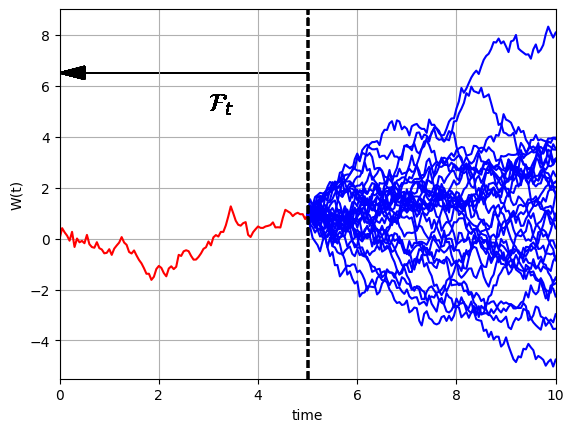
\includegraphics[width=0.8\linewidth]{images/filtration}
		\end{columns}
		
		\textbf{Martingale}: formally, a stochastic process is a martingale if
\begin{equation*} 
\mathbb{E}[X_{t+1}|\mathcal{F}_t] = X_t
\end{equation*}
or the conditional expectation of the next value in the sequence is equal to the present value, regardless of all prior values. 
It can be imagined as a \emph{drift-less} process
		\begin{equation*}
			dX = \cancel{\mu dt} + \sigma dW
		\end{equation*}
	\end{frame}

\section{Risk Neutral Pricing}
\begin{frame}{Risk Neutral Pricing Foundations}
	Harrison and Pliska proved and formalized the following results:
	\begin{itemize}
		\item \textbf{The market is free of arbitrage if (and only if) there exists an \textcolor{red}{equivalent martingale measure} (EMM) (i.e. a risk-neutral measure).}
	\end{itemize}
	\vfill
\end{frame}

\begin{frame}{Risk Neutral Pricing Foundations}
	\begin{itemize}
		\item Arbitrage opportunities rarely exist in practice. If and when they do, gains are extremely small, and are typically short-lived and difficult to spot. \textcolor{red}{Arbitrage exclusion in the mathematical model is close enough to reality}.
		\item An \textcolor{red}{equivalent martingale measure} $\mathbb{Q}$ is a probability measure on the space $\Omega$ such that
		\begin{enumerate}
			\item $\mathbb{Q}$ is equivalent to $\mathbb{P}$ (real world measure);
			\item for any asset $A$ and for each time $t$, $0\le t\le T$ there exists a price $\pi_t$
			\begin{equation*}
				\pi_t = \expect{Q}[D(t,T)V_A|\mathcal{F}_t]
			\end{equation*}
			which is a $\mathbb{Q}$-martingale.
		\end{enumerate}
	\end{itemize}
\end{frame}

\subsection{Risk Neutral Measure}
\begin{frame}{Risk Neutral Measure}
\begin{itemize}
\item  The difference between real world and risk neutral measures is in the treatment of the market price of risk.
\item If you tried to estimate the anticipated value of a stock based on how likely it is to go up or down, considering unique factors or market conditions that influence that specific asset, you would be including risk into the equation and, thus, would be looking at \textcolor{red}{real or physical probability}.
\item The \textcolor{red}{risk neutral measure}, instead, allows determination of a market-consistent value without making any assumption about the market price of risk. That is useful because the price of risk is not directly observable, but the market prices used to calibrate a risk-neutral generator are.
\item The risk neutral measure is a direct consequence of no arbitrage assumption. It is an \emph{implied probability distribution} from observable prices of tradable instruments, and used to determine \textcolor{red}{objective fair prices} for a financial instrument.
\end{itemize}
\end{frame}

\begin{frame}{Risk Neutral Pricing Foundations}
	Harrison and Pliska proved and formalized the following results:
	\begin{itemize}
		\item The market is free of arbitrage if (and only if) there exists an \textcolor{red}{equivalent martingale measure} (EMM) (i.e. a risk neutral measure).
		\item \textbf{The market is complete if and only if the martingale measure is unique.}
		
		(Note that market completeness means that any contingent claim can be replicated by a portfolio, or in other words that every asset in every possible state of the world has a price.)
	\end{itemize}
	\vfill
\end{frame}

%\begin{frame}{Summary of Basic Definitions}
%	\begin{itemize}
%		\item The market is complete if and only if the martingale measure is unique.
%		\item In a complete and arbitrage-free market the price of any derivative is uniquely given, either by the value of the associated replicating strategy, or by the expectation of the discounted payoff under the risk-neutral measure
%		\begin{equation}
%			\Pi_t = \mathbb{E}^{\mathcal{Q}^0}[D(t,T)V_A|\mathcal{F}_t]
%			\label{eq:risk_neutral_pricing}
%		\end{equation}
%	\end{itemize}
%\end{frame}

%\begin{frame}{Martingale}
%	\begin{block}{Definition}
%		A \textcolor{red}{$\mathcal{F}_t$-martingale} is a (integrable and adapted) stochastic process which models a fair game with the following remarkable feature
%		\begin{equation}
%			\mathbb{E}[X_t|\mathcal{F}_s] = X_s
%		\end{equation}
%		so the best prediction for the future value $X_t$, given the knowledge $\mathcal{F}_s$ at time $s$ is the value at time $s$ itself, $X_s$.
%	\end{block}
%	%	\begin{block}{Properties}
%		\begin{itemize}
%			\item If $X_t$ is a stochastic process with diffusion coefficient $\sigma_t$, such that %which satisfies $\mathbb{E}\left[\left(\int_0^T\sigma^2_s ds\right)^{\frac{1}{2}}\right]<\infty$, and SDE 
%			$dX_t=\mu_t dt+\sigma_t dW_t$, then 
%			\begin{equation*}
%				X\text{ is a martingale } \iff X\text{ is drift-less } (\mu_t=0)
%			\end{equation*}
%		\end{itemize}	
%	\end{frame}

%\begin{frame}{Equivalent Martingale Measure}
%	\begin{block}{Definition}
%		An \textcolor{red}{equivalent martingale measure} $\mathbb{Q}$ is a probability measure on the space $\Omega$ such that
%		\begin{enumerate}
%			\item $\mathbb{Q}$ is equivalent to $\mathbb{P}$;
%			\item for any asset $A$ and for each time $t$, $0\le t\le T$ there exists a price $\pi_t$
%			\begin{equation*}
%				\pi_t = \expect{Q^0}[D(t,T)V_A|\mathcal{F}_t]
%			\end{equation*}
%			\item the "discounted asset price" is a $\mathbb{Q}$-martingale
%			\begin{equation*}
%				\pi_u = \expect{Q^0}[D(0,t)V_A(t)|\mathcal{F}_u], \quad\text{with }(t>u)
%			\end{equation*}
%		\end{enumerate}
%	\end{block}
%\end{frame}

\begin{frame}{Risk Neutral Pricing Foundations}
	Harrison and Pliska proved and formalized the following results:
	\begin{itemize}
		\item The market is free of arbitrage if (and only if) there exists an \textcolor{red}{equivalent martingale measure} (EMM) (i.e. a risk-neutral measure).
		\item The market is complete if and only if the martingale measure is unique;
		\item \textbf{In a complete and arbitrage-free market the price of any derivative is uniquely given, either by the value of the associated replicating strategy, or by the expectation of the discounted payoff under the risk-neutral measure}
		\begin{equation}
			\Pi_t = \expect{Q}[D(t,T)V_A|\mathcal{F}_t]
			\label{eq:risk_neutral_pricing}
		\end{equation}
	\end{itemize}
\end{frame}

\begin{frame}{What is the Monte Carlo Technique ?}
\begin{itemize}
	\item Our main goal is to compute prices with \cref{eq:risk_neutral_pricing}, which may not always be analytically solvable.
	\item In addition, many stochastic factors (stock prices, interest rates\ldots), influence the result, making predictions challenging. 
	\item \textbf{The Monte Carlo simulation technique} is the right tool to tackle this kind of  problems.
	\item It is a probability-based simulation method which exploits random sampling to analyze uncertain outcomes.
	\item Instead of relying on single point estimates, \emph{it generates multiple scenarios based on probability distributions}. 
	\item This allows to assess the range of potential outcomes, not only a single average, providing a more comprehensive understanding of the problem in hand.
\end{itemize}
\end{frame}

\begin{frame}{Monte Carlo in Practice}
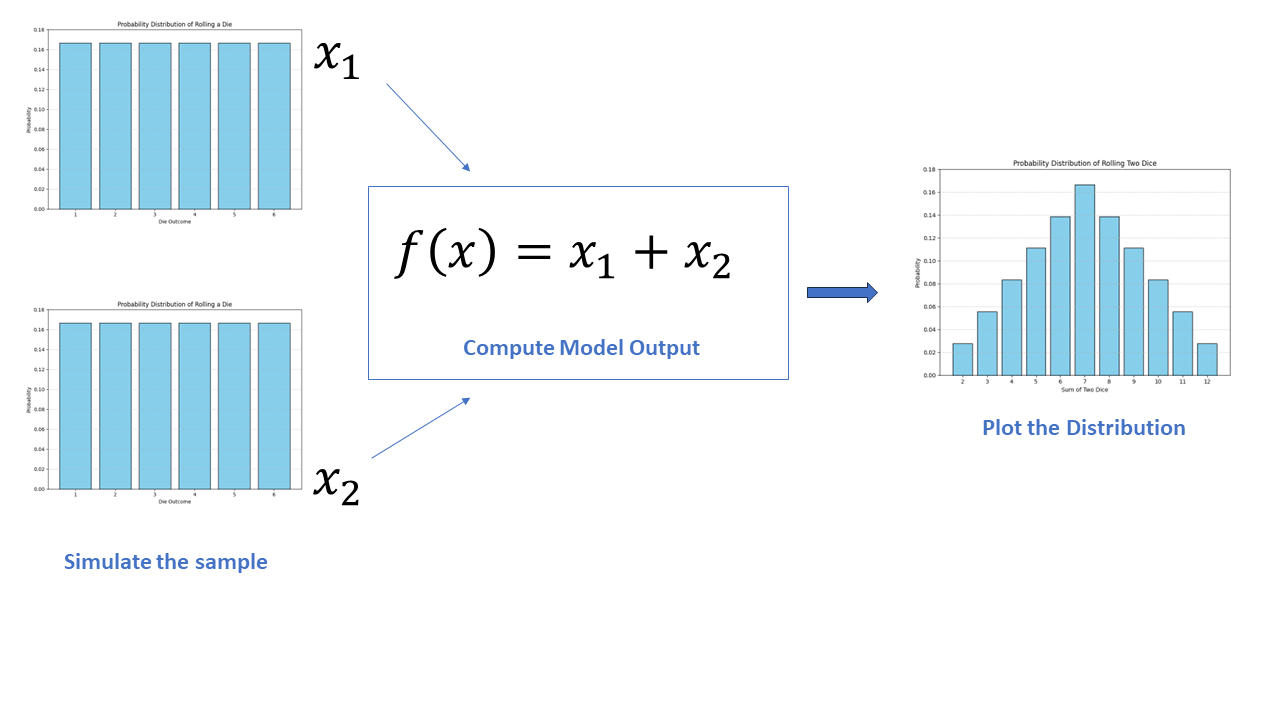
\includegraphics[width=1.0\linewidth]{images/monte_carlo_simulation}
\end{frame}


\begin{frame}[fragile]{Monte Carlo in Practice}
\begin{columns}
	\column{0.5\linewidth}
\begin{mintedbox}{python}[break at=.8\textheight]
import numpy as np
import matplotlib.pyplot as plt

num_trials = 10000

sums = []
for _ in range(num_trials):
    rolls = np.random.randint(1, 7, size=2)
    total_sum = np.sum(rolls)
    sums.append(total_sum)

plt.figure(figsize=(10, 6))
plt.hist(sums, bins=np.arange(2, 14) - 0.5, density=True, alpha=0.7, 
         color='skyblue', edgecolor='black', label='Simulated Sums')
\end{mintedbox}
    \column{0.5\linewidth}
    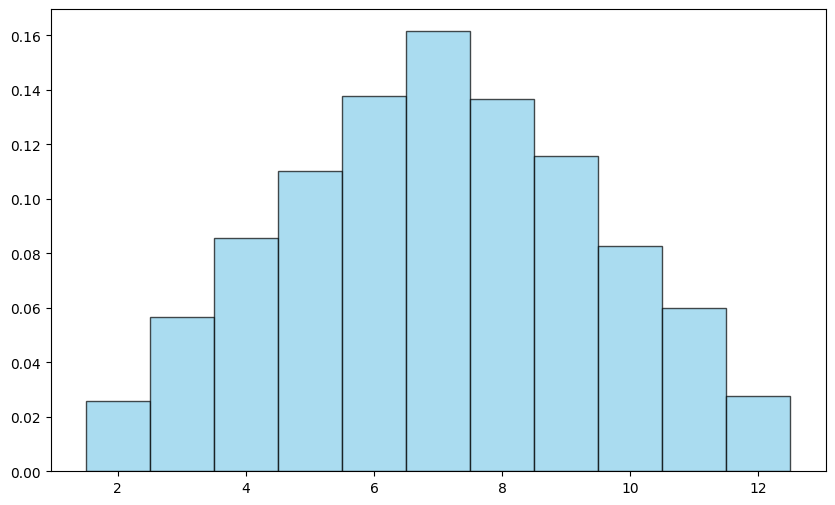
\includegraphics[width=0.8\linewidth]{images/sum_two_dice}
\end{columns}
\end{frame}

\begin{frame}{Central Limit Theorem}
\begin{block}{Theorem}
The \textbf{Central Limit Theorem} states: \emph{the sampling distribution of the mean is normally distributed, as long as the sample size is large enough}.
	
\begin{enumerate}
    \item the best estimate of a quantity given by MC experiments is the \textbf{mean} of the simulation results;
    \item with a larger sample size, your sample mean is \textbf{more likely to be close to the population mean} (more precise estimate).
\end{enumerate}
\end{block}

\begin{itemize}
\item The \emph{population} is the entire dataset collected based on a common feature common characteristics which can be used for statistical purposes (e.g. the dataset with the weights of all the fishes in the sea).
\item The \emph{sample} is a subset of a population with fewer data points i.e. data selected randomly from a population. The \emph{sample mean} is the average value calculated on the sample dataset.
\end{itemize}
\end{frame}

\begin{frame}[fragile]{Central Limit Theorem Example}
\begin{columns}
    \column{0.5\linewidth}
         \begin{table}
            \centering
            \begin{tabular}{cc}
                Size & Estimated Mean \\
                \hline
                10 & $5.011 \pm 0.708$  \\
                100 & $5.007 \pm 0.223$ \\
                1000 & $5.007 \pm 0.070$\\
            \end{tabular}
            \label{tab:my_label}
        \end{table}
    \column{0.5\linewidth}
        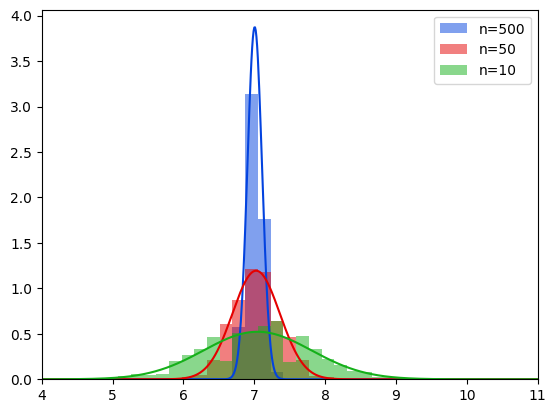
\includegraphics[width=0.8\linewidth]{images/sample_mean}
\end{columns}
\begin{itemize}
    \item The resulting "improvement" can also be quantified:
    \begin{equation}
    \cfrac{0.708}{0.223} = 3.175 \simeq \sqrt{\cfrac{100}{10}} = 3.162
    \label{eq:clt}
    \end{equation}
    which tells us that \textbf{the uncertainty scales as the square root of the sample size}.
\end{itemize}
\end{frame}

\begin{frame}{Central Limit Theorem Example}
\begin{itemize}
    \item This shows that no matter what our population distribution curve is, the sample means will always follow Gaussian Distribution.
    \item Sample sizes equal to or greater than 30 are considered sufficient for the theorem to hold but that might not be always necessary. In our example, we can observe that we get a Gaussian Distribution with a sample size of 10 or 20 too.
    \item Statistical analysis of the data of the entire population are practically impossible in almost all cases. Sample data of any population can be used to draw conclusions about the overall population using CTL as we know that sample means are always normally distributed!!!!
\end{itemize}
\end{frame}

\begin{frame}{Stochastic Simulation}
\begin{itemize}
    \item Consider a generic SDE of the form  
        \begin{equation*}
        dX(t) = \mu(t,X(t))dt + \sigma(t,X(t))dW(t) 
        \end{equation*}
    \item The simulation of $X(t)$ follows the \emph{Euler Scheme}: starting from the \textbf{known} value of $X(t_0)$ simply compute $X(t_0 +\Delta t)$ using the given SDE:
        \begin{equation*}
            X(t_0+\Delta t) = X(t_0) + dX(t)
        \end{equation*}
    \item Setting $\Delta t$ to a "reasonable" value, $dX$ can be computed by evaluating the two coefficients $\mu(t_0,X(t_0))$ and $\sigma(t_0,X(t_0))$; $dW$ is a standard Brownian motion, so its value can be obtained by sampling from a standard normal $Z=\mathcal{N}(0,1)$:
        \begin{equation*}
            X(t_{i+1}) = X(t_i) + \mu(t_i,X(t_i))\Delta t + \sigma(t_i,X(t_i))\sqrt{\Delta t}Z 
        \end{equation*}
    \end{itemize}
\end{frame}

\begin{frame}[fragile]{Brownian Motion Example}

In the specific case of a simple Brownian motion the dynamics is given by $dW = \sqrt{dt}\mathcal{N}(0,1)$ so
\begin{equation}
W(t+\Delta t) = W(t) + \sqrt{\Delta t}Z \implies
W(t) = W(t_0) + \sum_{t_0}^{t} \sqrt{\Delta t}Z
\label{eq:bm_evolution}
\end{equation}

\begin{block}{\texttt{Python} Digression}
For the rest of the course we are going to show \texttt{python} examples using a framework we have developed, mostly hiding the underlying technical details.

For the BM example I would like to show how usually this problems are tackled in \texttt{python} analyzing once and for all the code.
\end{block}
\end{frame}

\begin{frame}{Brownian Motion Example}
\begin{itemize}
    \item \texttt{Python} is not that great when dealing with complex calculation; the trick that is usually used in these cases is to move to \emph{linear algebra} using dedicated libraries (e.g. \texttt{numpy}) which are highly optimized for such calculations.
    \item The goal here is to simulate $N$ \emph{realizations} of a Brownian motion process with $m$ \textit{time steps} and initial value 0. 
    \item Instead of performing each single calculation for each realization and each time step, we are going to use matrices and perform bunch of operations at once.
    \item Let's start with a $(N\times m)$ matrix $[W_0]$
    $$
    [W_0] =
    \begin{bmatrix}
    W^1_0 & W^2_0 & \cdots & W^N_0 \\
    0 & 0 & \cdots & 0 \\
     &  & \vdots &   \\
    0 & 0 & \cdots & 0 \\
    \end{bmatrix}
    $$
    \end{itemize}
\end{frame}

\begin{frame}{Brownian Motion Example}
\begin{itemize}
    \item Then we can calculate each variation by sampling $N\times (m-1)$ times from the Normal distribution and create a second matrix 
    $$
    [dW] =
    \begin{bmatrix}
    0 & 0 & \cdots & 0 \\
    dW^1_1 & dW^2_1 & \cdots & dW^N_1 \\
     &  & \vdots &   \\
    dW^1_{m} & dW^2_{m} & \cdots & dW^N_{m} \\
    \end{bmatrix}
    $$  
    \item Let's sum 
    $$[W] = [W_0] + [dW] =
    \begin{bmatrix}
    W^1_0 & W^2_0 & \cdots & W^N_0 \\
    dW^1_1 & dW^2_1 & \cdots & dW^N_1 \\
     &  & \vdots &   \\
    dW^1_{m} & dW^2_{m} & \cdots & dW^N_{m} \\
    \end{bmatrix}
    $$  
\end{itemize}
\end{frame}

\begin{frame}{Brownian Motion Example}
\begin{itemize}
    \item Finally, remembering the \cref{eq:bm_evolution}, we can obtain the Brownian motion evolution in each realization by simply summing up all the columns in $[W]$

\[\left[
\begin{array}{cccc}
W^1_0 & W^2_0 & \cdots & W^N_0 \\
\downarrow & \downarrow & \cdots & \downarrow \\
dW^1_1 & dW^2_1 & \cdots & dW^N_1 \\
\downarrow & \downarrow & \vdots & \downarrow \\
dW^1_{m} & dW^2_{m} & \cdots & dW^N_{m} \\
\downarrow & \downarrow & \cdots & \downarrow \\
W^1_0+\sum\limits_{i=1}^{m} dW^1_i & W^2_0+\sum\limits_{i=1}^{m} dW^2_i & \cdots & W^N_0+\sum\limits_{i=1}^{m} dW^N_i
\end{array}\right]
\]
\end{itemize}
\end{frame}

\begin{frame}[fragile]{Brownian Motion Example}
\begin{columns}
	\column{0.55\linewidth}
\begin{mintedbox}{python}[break at=.9\textheight]
import numpy as np

N = 10; m = 100; W0 = 0
W = np.zeros(shape=(m, N))
W[0, :] = W0
W[1:, :] = np.random.normal(size=(m-1, N))*np.sqrt(1/m)
W = np.cumsum(W, axis=0)
\end{mintedbox}
    \column{0.4\linewidth}
    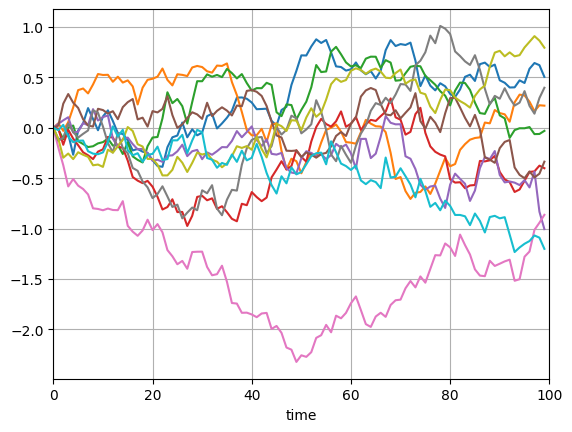
\includegraphics[width=1.\linewidth]{images/bm_realizations}
\end{columns}
\begin{block}{Important}
Those are 10 out of an infinite number of \textbf{possible} realizations of a  BM: as a stochastic process it is impossible to know how it will develop in the future.

A statistical analysis of a stochastic process necessarily involves the \emph{expected value} ($\mathbb{E}$) (i.e. the mean) of the random process.
\end{block}
\end{frame}

\begin{frame}{Geometric Brownian Motion Example}
\begin{itemize}
    \item Similarly to what have been done before we can simulate the evolution of a Geometric Brownian Motion (GBM), the random process that usually models stocks
    \begin{equation*}
        dS(t) = \mu S(t) dt + \sigma S(t) dW(t)
    \end{equation*}
    where: $\mu$ is the drift term (expected return), $\sigma$ is the volatility (standard deviation of the returns), and $dW$ is a standard Wiener process (Brownian motion).
    \item The proceed we can either implement again the Euler scheme or directly use the analytical solution of the GBM
    \begin{equation*}
        S(t) = S(0)e^{(\mu-\frac{1}{2}\sigma^2)t+\sigma W_t}
    \end{equation*}
    where $S_0$ is the initial price of the asset at time.
    \item Notice that the logarithm of $S(t)$ follows a normal distribution:
    \begin{equation*}
        \ln(S(t)) = \mathcal{N}\left(\left[\ln(0) +\left(\mu +\cfrac{\sigma^2}{2}\right)t \right], \sigma^2 t\right)
    \end{equation*}
\end{itemize}
\end{frame}

\begin{frame}[fragile]{Geometric Brownian Motion Example}
\begin{itemize}
    \item Let's see the results of such a simulation for a 8-months (with daily steps) period with initial value $S_0=100$, $\mu=0.005$, and $\sigma=0.05$.
\end{itemize}

\begin{columns}
	\column{0.55\linewidth}
\begin{mintedbox}{python}[break at=.9\textheight]
import tensorquant as tq
import tensorflow as tf

gbm = tq.GeometricBrownianMotion(mu=0.005, sigma=0.05, x0=100)

n_path = 10
timesteps = 240
Z = tf.random.normal((n_path, timesteps), seed=12, dtype=tf.dtypes.float64)
t = tf.Variable(8, dtype=tf.float64)
S_t = gbm.evolve(t, Z)
\end{mintedbox}
    \column{0.4\linewidth}
    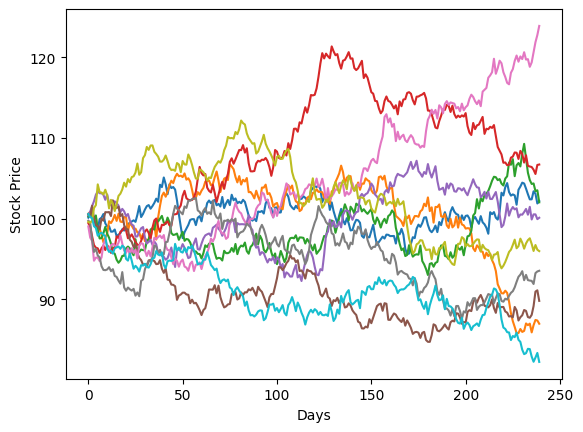
\includegraphics[width=1.1\linewidth]{images/gbm_realizations}
\end{columns}
If you want to try this code remember to install \texttt{tensorquant} with the command \texttt{pip install tensorquant}.
\end{frame}

\begin{homework}
\begin{frame}{\textcolor{white}{Homework}}
\begin{itemize}
\item[white]  You have determined the value of an interest rate derivative with a Monte Carlo simulation involving 50 scenarios which results in a contract value of 1.2 M€ $\pm$ 5\%. Unfortunately, your boss asks you to determine more precisely the derivative value. If you have to meet him in 1 hour and each simulation lasts about 2.5 sec., what is the highest precision you can achieve ?
\item[white] Consider the process $Y(t) = 2^{W(t)}$, where $\{W(T):t\geq 0\}$ is a standard Brownian motion. Is this a martingale ?
\item[white]  Show that the exponential SDE
\begin{equation*}
dX_t = A_t X_tdW_t,\quad X_0=x_0
\end{equation*}
has the following solution
\begin{equation*}
X_t = x_0 e^{-\frac{1}{2}\int_0^t A_0^2 ds+\int_0^t A_s dB_s}
\end{equation*}
\end{itemize}
\textcolor{white}{Exercises for this part involves: SDE solving, martingale definition, Ito's lemma, and a bit of Monte Carlo theory.}
\end{frame}
\end{homework}

\end{document}
